This chapter includes the Alloy code, used to describe and check the consistency of our model (see also the class diagram at \ref{subsec:Class Diagram})using a formal notation and to provide examples of the possible worlds generated by the Alloy analyzer tool.
\newline
We've described the domain of our model and his main properties (all modeling assumptions are described directly into the alloy code below) and we've also modeled some main operations to be provided by the system-to-be.
Therefore we've proven the consistency of our model and we've used the results to refine our specifications contained into this document; during the alloy's modeling effort we've point out some flaws of our assumptions and of our UML models and so we've fixed it.
\section{Model}
	\lstinputlisting[language=alloy]{4-FormalAnalysisUsingAlloy/Travlendar+.als}

\section{Proof of Consistency}
		\noindent\makebox{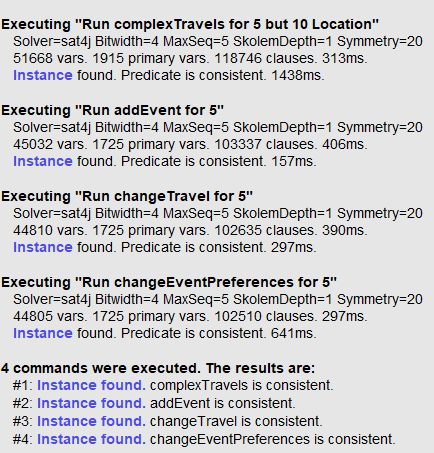
\includegraphics{alloy_worlds/Alloy_Results.png}}
	
\section{Worlds obtained}
	\subsection{World 1}
	\noindent\makebox[\textwidth]{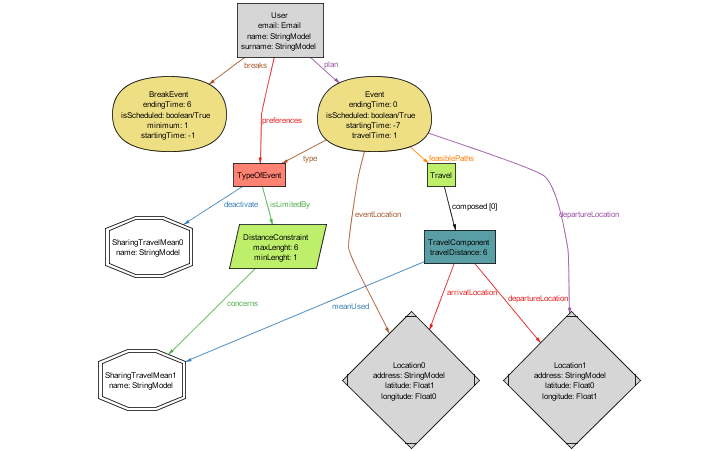
\includegraphics[scale=0.50]{alloy_worlds/alloy_model_1.png}}
	
	\subsection{World 2}
	\noindent\makebox[\textwidth]{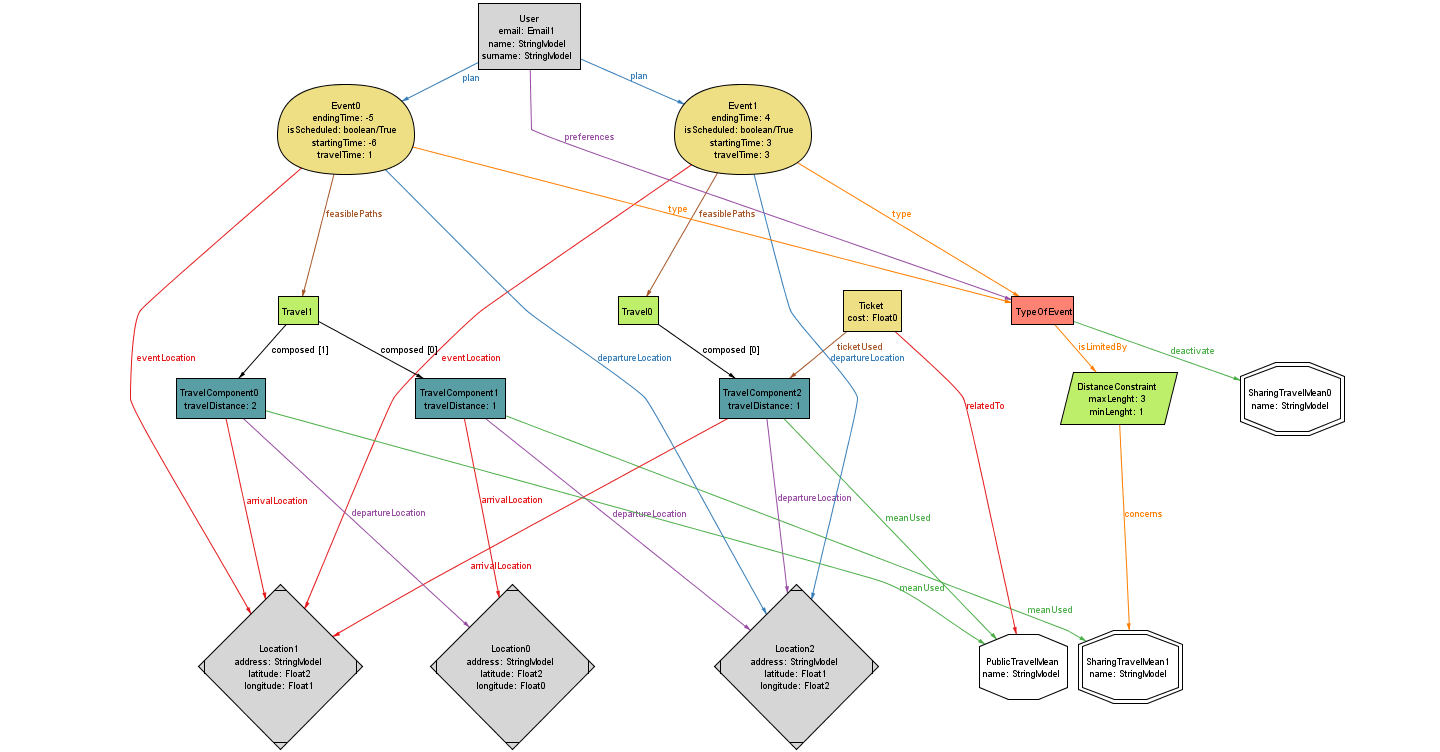
\includegraphics[width=\paperwidth,height=\paperheight,keepaspectratio]{alloy_worlds/alloy_model_2.png}}
	
	\subsection{World 3}
\begin{figure}
\begin{center}
		\vspace*{-100pt}
		\hspace*{-50pt}
		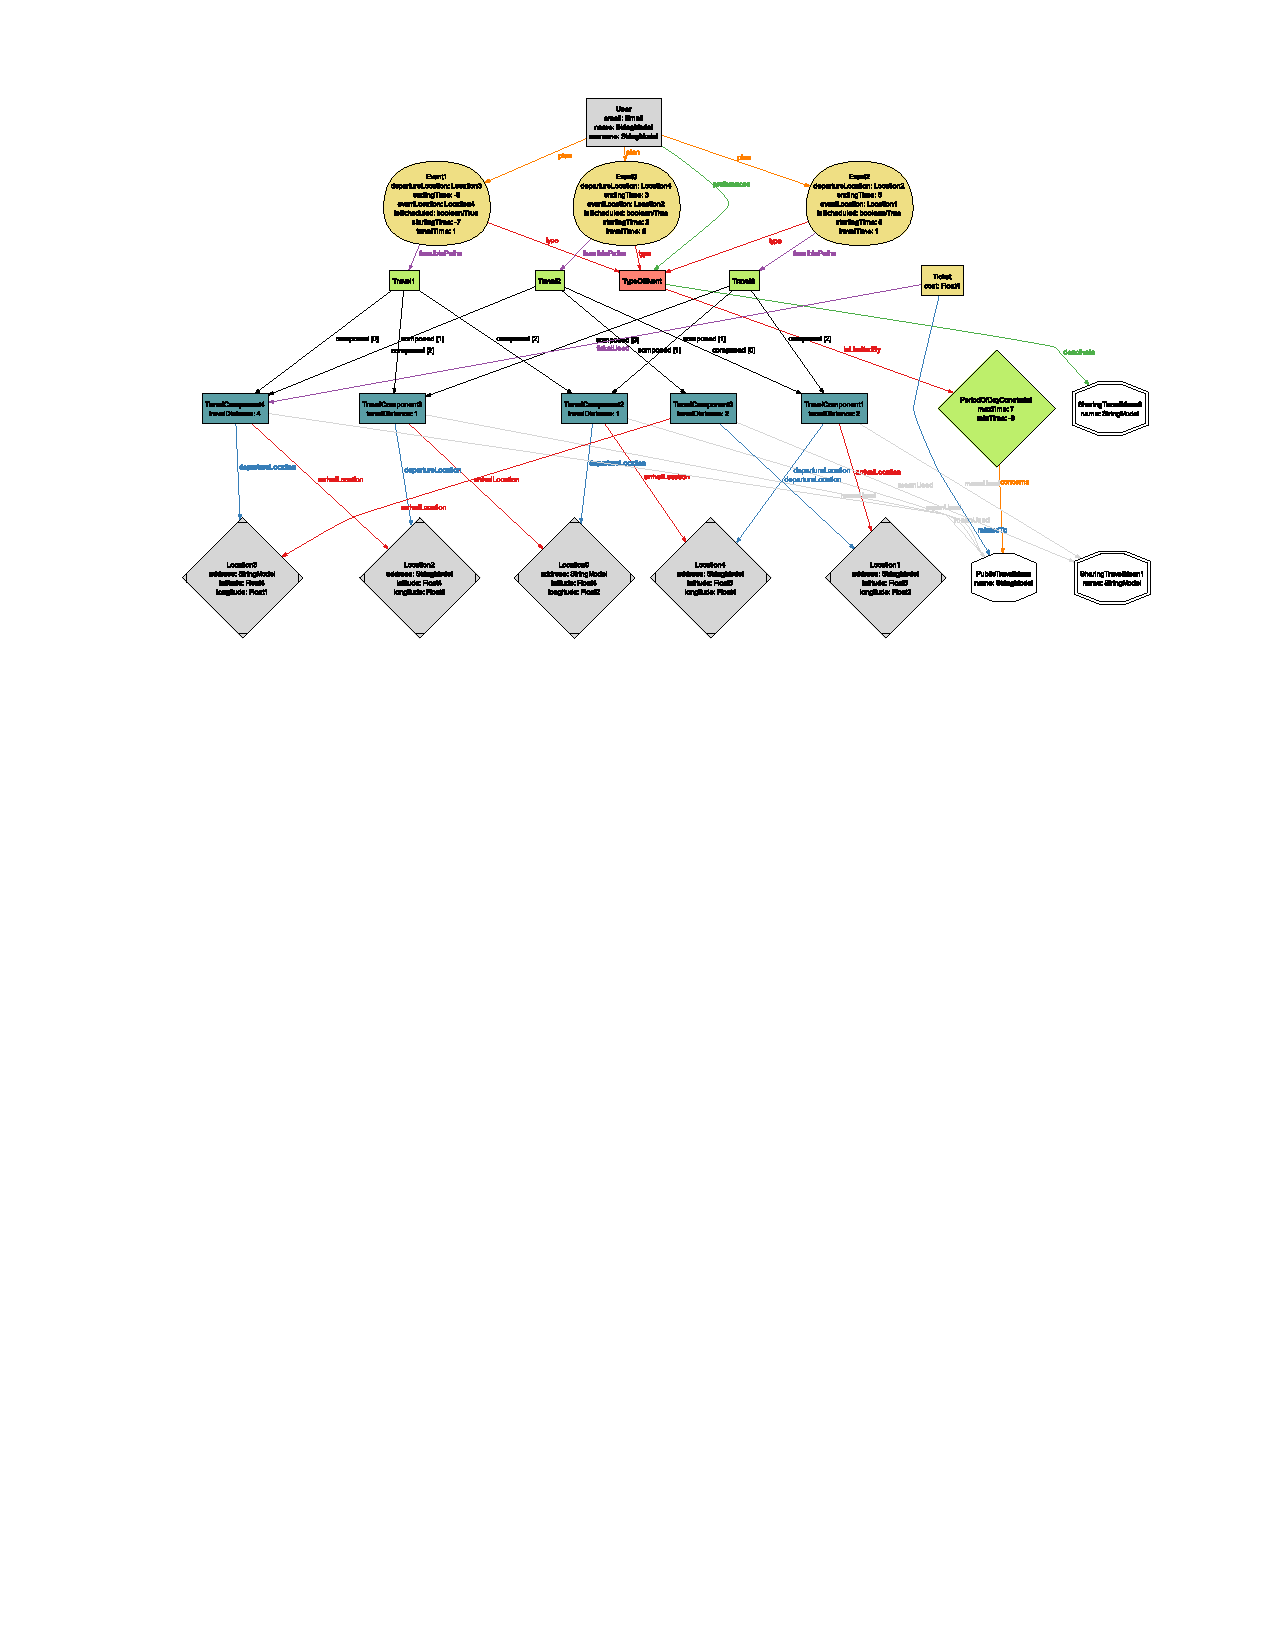
\includegraphics[width=925pt, angle= 90]{alloy_worlds/alloy_model_3.pdf}
		\label{class_diagram}
\end{center}
\end{figure}
	
	